
\documentclass[fleqn,addpoints]{exam}
\usepackage{amsmath}
\usepackage{graphicx}
\usepackage{booktabs}
\usepackage{float}
\usepackage{caption}
\usepackage{polynom}
\usepackage{mdwlist}
\usepackage{cancel}

\usepackage{unitsdef} 
\newunit{\inch}{in}
\newunit{\mile}{mile}
\newunit{\mph}{mph}
\newunit{\foot}{ft}
\newunit{\knot}{knot}
\newunit{\gallon}{gallon}

\printanswers
\bracketedpoints
\everymath{\displaystyle}


% \begin{figure}[H]
%   \centering
%   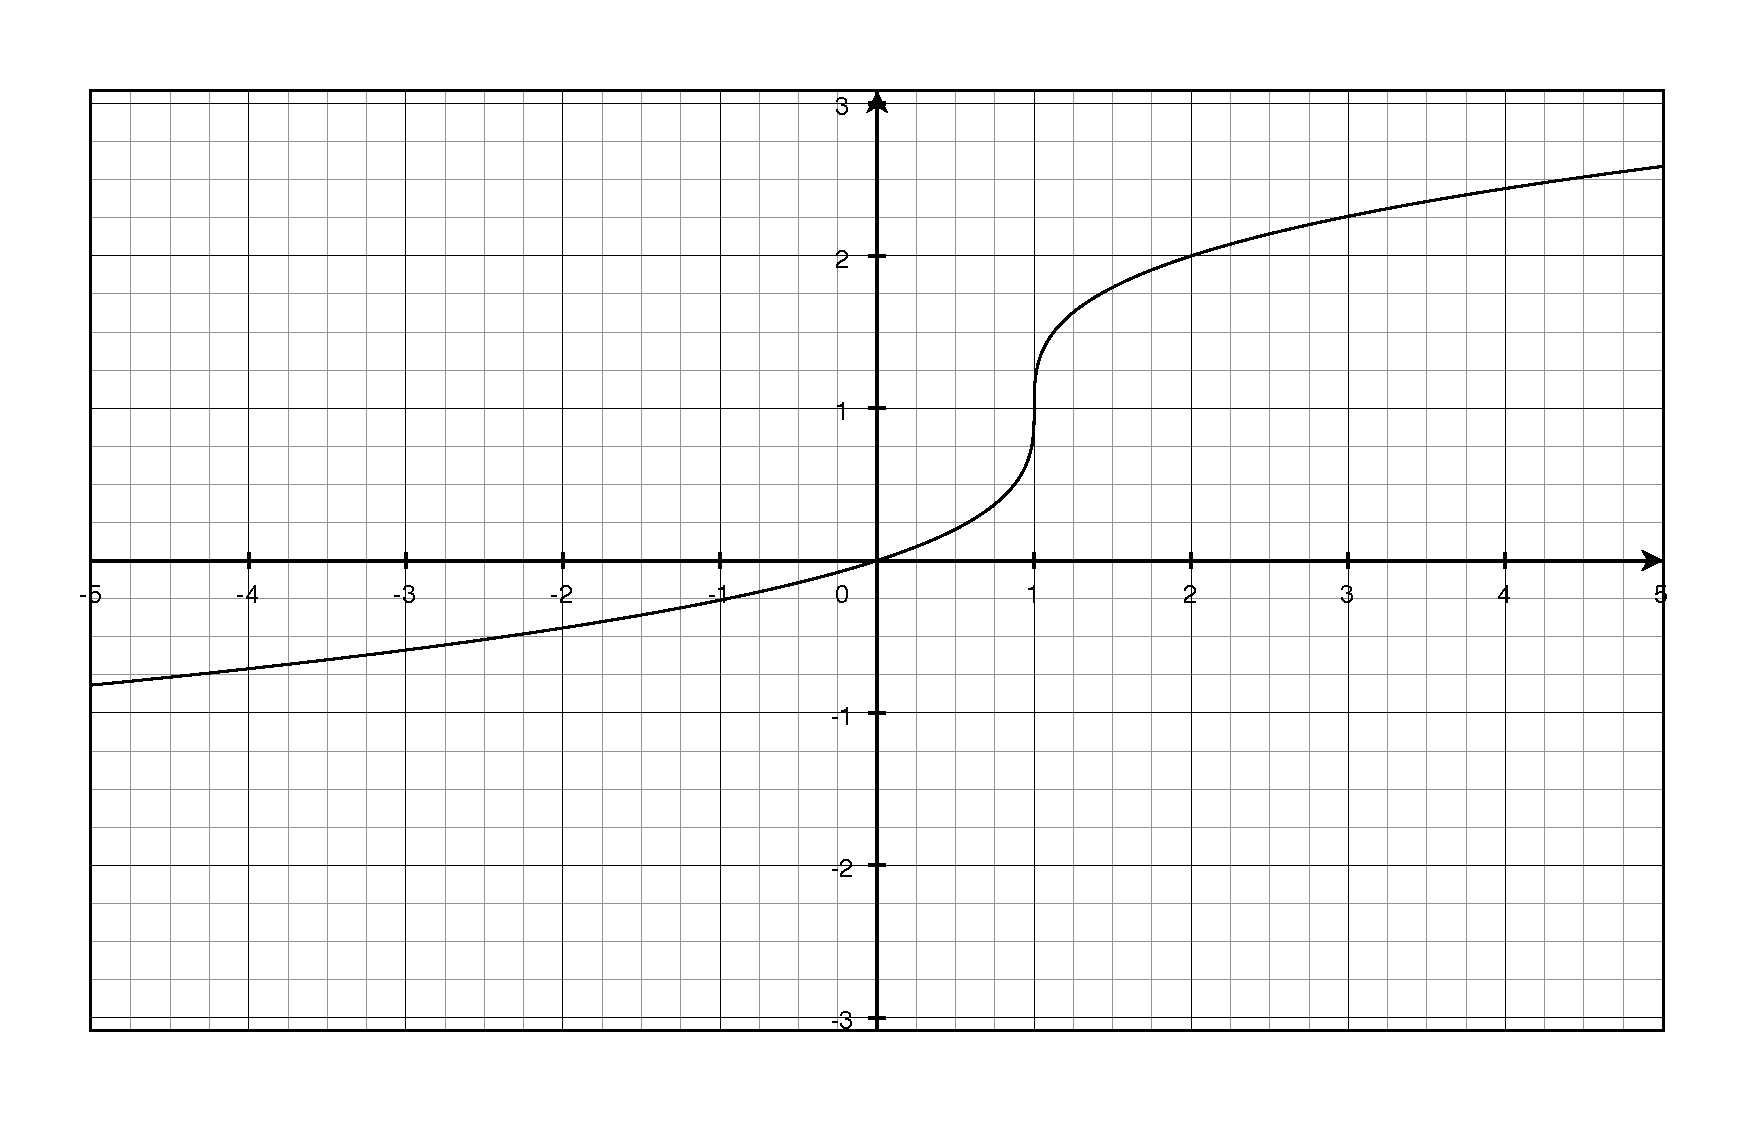
\includegraphics[scale=.3]{question7.eps}
%   \caption*{Question 7}
% \end{figure}

% \begin{tabular}{cc}
% \toprule
% period & amplitude \\
% \midrule
%   $\pi$ & $2$ \\
% \bottomrule
% \end{tabular}


%% \ifprintanswers
%% \usepackage{2in1, lscape}
%% \fi

\title{Math 263A Exam Two \\ Chapter 4}
\date{June 6, 2012}

\author{}

\begin{document}

\maketitle  

\ifprintanswers
\else
\vspace{0.2in}
\makebox[\textwidth]{Name:\enspace\hrulefill}
\vspace{0.2in}

\begin{center}

\gradetable[h][pages]

\vspace{.5 cm}

\bonusgradetable[h][pages]
\end{center}

% \tableofcontents

\fi

\ifprintanswers
\else
\pagebreak
\fi

\begin{questions}

\uplevel{\section{Minimum/Maximum}}
\uplevel{For questions \ref{min_max_range:first} to \ref{min_max_range:last}, find the minimums and maximums (if they exist) in the
  indicated range.}

\question[5]
\label{min_max_range:first}
\[
  f(x) = x^3  -3x + 1 \text{; range: } [0, 3]
\]

\begin{solution}[8 cm]
\begin{align*}
  f(x) &= x^3  -3x + 1 \\
  f'(x) &= 3x^2  -3 \\
\\
  3x^2  -3 &> 0 \\
  x^2  - 1 &> 0 \\
  (x + 1)(x - 1) &> 0 \\
  x < -1 &\text{ or } x > 1 \\
\end{align*}

\begin{tabular}{rrl}
\toprule
x & f(x) & min/max \\
% \midrule
0 & 1 & \\
1 & -1 & min \\
3 & 19 & max \\
\bottomrule
\end{tabular}

\end{solution}

\ifprintanswers
\pagebreak
\fi

\question[5]
\label{min_max_range:last}
\[
  f(x) = \frac{1}{x} \text{; range: } (0, 1]
\]

\begin{solution}[6 cm]
\begin{align*}
  f(x) &= \frac{1}{x} \\
  f'(x) &= \frac{-1}{x^2} \\
\end{align*}

$f'$ is always negative, so $f$ is always decreasing.  The minimum value is $(1, 1)$.  There isn't a maximum, because 0
isn't in the range.

\end{solution}

%% \question[5]
%% \label{min_max_range:last}
%% \[
%%   f(x) = \sqrt{9 - x^2} \text{; range: } [-1, 2]
%% \]

%% \begin{solution}[7 cm]
%% \end{solution}

%% \question[7]
%% \label{min_max_range:first}
%% \[
%%   f(x) = \sin x + \cos x \text{; range: } [0, \pi]
%% \]

\ifprintanswers
\else
\pagebreak
\fi

\uplevel{For questions \ref{local_min_max:first} to \ref{local_min_max:last}, find: (a) the local extrema and (b) the
  intervals on which $f$ is increasing/decreasing.}

\question[5]
\label{local_min_max:first}
\[
  f(x) = x^4 + 4x^3 + 4x^2
\]

\begin{solution}[7 cm]
\begin{align*}
  f(x) &= x^4 + 4x^3 + 4x^2 \\
  f'(x) &= 4x^3 + 12x^2 + 8x \\
\\
  4x^3 + 12x^2 + 8x &> 0 \\
  x^3 + 3x^2 + 2x &> 0 \\
  x(x^2 + 3x + 2) &> 0 \\
  x(x + 1)(x+2) &> 0 \\
\end{align*}

\begin{tabular}{lr}
\toprule
increasing     & $[-2, -1] \cup [0, \infty)$ \\
decreasing     & $(-\infty, -2] \cup [-1, 0]$ \\
local minimum  & $(-2, 0)$ and $(0, 0)$\\
local maximum  & $(-1, 1)$ \\
\bottomrule
\end{tabular}

\end{solution}

\ifprintanswers
\pagebreak
\fi

\question[7]
\label{local_min_max:last}
\[
  f(x) = \frac{2x}{x^2 + 1}
\]

\begin{solution}[6 cm]
\begin{align*}
  f(x) &= \frac{2x}{x^2 + 1} \\
  f'(x) &= \frac{(x^2 + 1) \cdot 2 - 2x (2x)}{(x^2 + 1)^2} \\
        &= \frac{-2x^2 + 2}{(x^2 + 1)^2} \\
\\
  -2x^2 + 2 &> 0 \\
  1 - x^2 &> 0 \\
\end{align*}

\begin{tabular}{lr}
\toprule
increasing     & $[-1, 1]$ \\
decreasing     & $(-\infty, -1] \cup [1, \infty)$ \\
local minimum  & $(-1, -1)$ \\
local maximum  & $(1, 1)$ \\
\bottomrule
\end{tabular}

\end{solution}

%% \begin{solution}[3 cm]
%% \end{solution}

%% \question[5]
%% \[
%%   f(x) = 10x^3(x-1)^2
%% \]

%% \question[7]
%% \label{local_min_max:last}
%% \[
%%   f(x) = x + \frac{1}{x}
%% \]

%% \begin{solution}[6 cm]
%% \end{solution}

\ifprintanswers
\else
\pagebreak
\fi

\uplevel{\section{Concavity}}
\uplevel{For questions \ref{concavity:first} to \ref{concavity:last}, find the (a) inflection points and (b) intervals on which $f$
  is concave up/down.}

\question[5]
\label{concavity:first}
\[
  f(x) = x^4 - 6x^3 + 7x - 5
\]

\begin{solution}[8 cm]
\begin{align*}
  f(x) &= x^4 - 6x^3 + 7x - 5 \\
  f'(x) &= 4x^3 - 18x^2 + 7 \\
  f''(x) &= 12x^2 - 36x \\
\\
  12x^2 - 36x &> 0 \\
  x^2 - 3x &> 0 \\
  x(x - 3) &> 0 \\
\end{align*}

\begin{tabular}{lr}
\toprule
concave up     & $(-\infty, 0) \cup (3, \infty)$ \\
concave down   & $(0, 3)$ \\
\bottomrule
\end{tabular}

\end{solution}

\question[5]
\[
  f(x) = x - 3x^{1/3}
\]

\begin{solution}[8 cm]
\begin{align*}
  f(x) &= x - 3x^{1/3} \\
  f'(x) &= 1 - x^{-2/3} \\
  f''(x) &= \frac{2}{3} x^{-5/3} \\
\\
  \frac{2}{3} x^{-5/3} &> 0 \\
  x &> 0 \\
\end{align*}

\begin{tabular}{lr}
\toprule
concave up   & $(0, \infty)$ \\
concave down & $(-\infty, 0)$ \\
\bottomrule
\end{tabular}

\end{solution}

%% \question[8]
%% \[
%%   f(x) = \left( \frac{x}{x+1} \right)^2
%% \]
%% \begin{solution}[8 cm]
%% \end{solution}

\question[8]
\label{concavity:last}
\[
  f(x) = \cos^2 x \text{ on } [0, \pi]
\]

\begin{solution}
\begin{align*}
  f(x) &= \cos^2 x \\
  f'(x)  &= -2 \sin \cos x \\
  f''(x) &= -2 (\cos^2 x - \sin^2 x) \\
         &= 2 (\sin^2 x - \cos^2 x) \\
\\
  2(\sin^2 x - \cos^2 x) > 0 \\
  (\sin x + \cos x) (\sin x - \cos x) > 0 \\
\end{align*}

\begin{tabular}{lr}
\toprule
concave up   & $\left( \frac{\pi}{4}, \frac{3 \pi}{4} \right)$ \\
concave down & $\left(0, \frac{\pi}{4} \right) \cup \left(\frac{3 \pi}{4}, \pi \right)$ \\
\bottomrule
\end{tabular}

\end{solution}

\pagebreak

\uplevel{\section{Optimization}}

\question[15]

A cylindrical container with an open top is to hold $1 \meter^3$ of water.  Find the dimensions which require the least
amount of material to construct the container.

The equations for a cylinder are:
\begin{align*}
  V_{cylinder} &= \pi r^2 h \\
  A_{cylinder} &= 2 \pi r h \text{ (not including the top or bottom)} \\
\end{align*}

\begin{solution}
To minimize the amount of material required, we should  minimize the area of the cylender.  Including the bottom, the area is:
\[
    A = 2 \pi r h + \pi r^2
\]

To optimize we need an equation with only one variable.  We can get this by solving the volume equation for $h$ and
plugging this result into the area equation: 
\begin{align*}
  V &= \pi r^2 h \\
  1 &= \pi r^2 h \\
  h &= \frac{1}{\pi r^2} \\
\\
  A(r) &= 2 \pi r \cdot \frac{1}{\pi r^2} + \pi r^2 \\
       &= \frac{2}{r} + \pi r^2 \\
\\
  A'(r) &= \frac{-2}{r^2} + 2 \pi r \\
  \frac{-2}{r^2} + 2 \pi r &= 0 \\
  \pi r &= \frac{1}{r^2}  \\
  r &= \sqrt[3]{\frac{1}{\pi}} \\
\end{align*}


\end{solution}

\pagebreak


%% \question[10]
%% \label{optimization:last}
%%   At noon, ship A is 15 miles due north of ship B and is sailing south at 20 mph.  Ship B is sailing east at 10 mph.
%%   Find the time when the ships are closest together.

%% \begin{solution}
%% \end{solution}

%% \ifprintanswers
%% \else
%% \pagebreak
%% \fi

\uplevel{\section{Limits}}
\uplevel{For questions \ref{limit:first} to \ref{limit:last}, evaluate each limit.}

\question[5]
\label{limit:first}
\[
  \lim_{x \to -3^+} \frac{x}{x + 3}
\]
\begin{solution}[3 cm]
\[
  \lim_{x \to -3^+} \frac{x}{x + 3} = - \infty
\]
\end{solution}

%% \question[5]
%% \label{limit:first}
%% \[
%%   \lim_{x \to -3^+} \frac{2}{x + 3}
%% \]
%% \begin{solution}[3 cm]
%% \end{solution}

\question[5]
\label{limit:first}
\[
  \lim_{x \to 2^-} \frac{x - 1}{x^2(x - 2)}
\]
\begin{solution}[3 cm]
\[
  \lim_{x \to 2^-} \frac{x - 1}{x^2(x - 2)} = -\infty
\]
\end{solution}

\question[5]
\[
  \lim_{x \to \pi^-} \csc x
\]
\begin{solution}
\[
  \lim_{x \to \pi^-} \csc x = \lim_{x \to \pi^-} \frac{1}{\sin x} = \infty
\]
\end{solution}

\pagebreak


%% \question[5]
%% \[
%%   \lim_{x \to \infty} \frac{x^2 + 3x - 1}{2x^3 - 7x^2}
%% \]
%% \begin{solution}[4 cm]
%% \end{solution}

%% \question[5]
%% \[
%%   \lim_{x \to \infty} \frac{x + 3}{x^2 - x}
%% \]
%% \begin{solution}[2 cm]
%% \end{solution}

\question[5]
\[
  \lim_{x \to -\infty} \frac{2x^3 + 3x^2 - 1}{x^3 + 2x^2 + 5}
\]
\begin{solution}[5 cm]
\[
  \lim_{x \to -\infty} \frac{2x^3 + 3x^2 - 1}{x^3 + 2x^2 + 5} 
    = \lim_{x \to -\infty} \frac{2 + 3/x - 1/x^3}{1 + 2/x + 5/x^3} = 2 \\   
\]

\end{solution}


\question[7]
\label{limit:last}
\[
  \lim_{x \to \infty} \frac{6x}{\sqrt{4x^2 + 1}}
\]

\begin{solution}[5 cm]
\[
  \lim_{x \to \infty} \frac{6x}{\sqrt{4x^2 + 1}} = \lim_{x \to \infty} \frac{6}{\sqrt{4 + 1/x^2}} = 3
\]
\end{solution}


\ifprintanswers
\else
\pagebreak
\fi

\uplevel{\section{Graphing}}
 
%% \uplevel{For questions \ref{graph:first} to \ref{graph:last}, check for symmetry, find where the graph is
%%   increasing/decreasing and concave up/down, find local min/max, find asymptotes, and draw the graph.}

%% \vspace{0.5 cm}

%% \question[10]
%% \label{graph:first}

%% \[
%%   f(x) = x^3 + 3x^2 + 1
%% \]


%% \begin{solution}[7 cm]
%% \end{solution}

%% \begin{figure}[H]
%%   \centering
%%   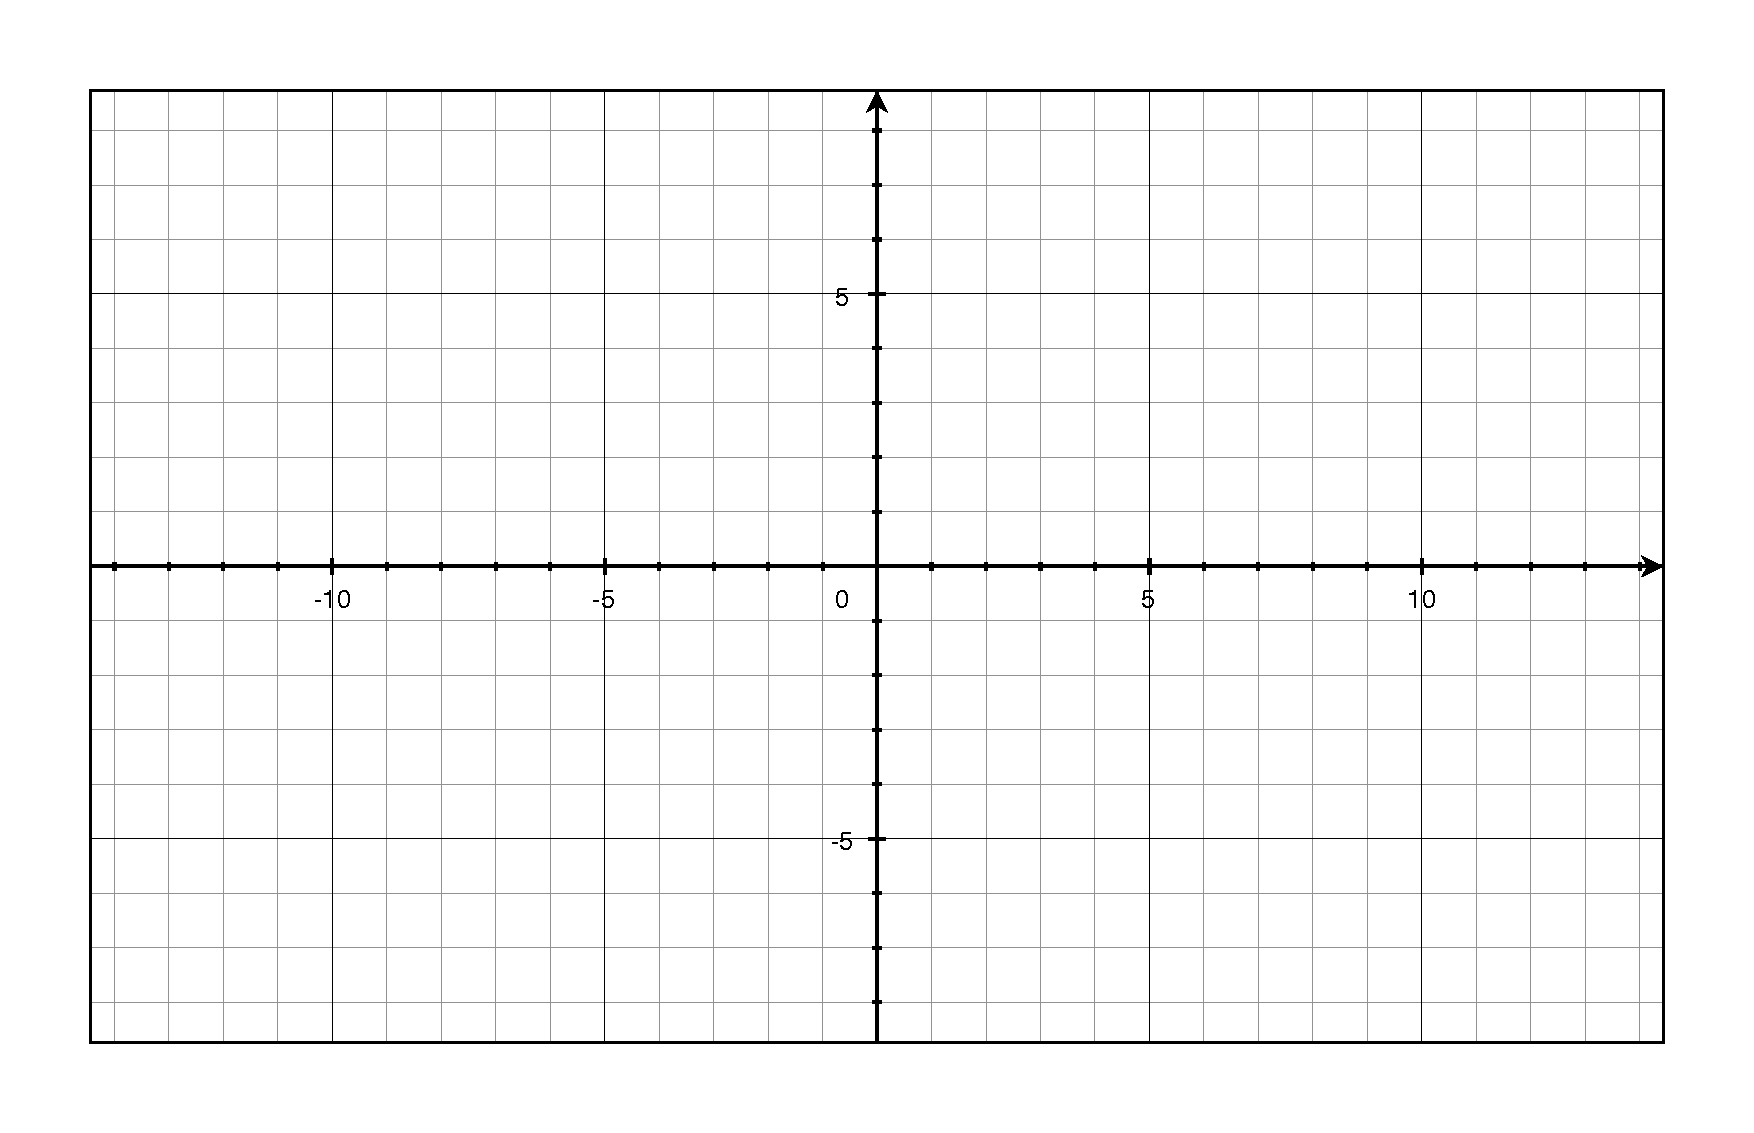
\includegraphics[scale=.5]{empty_grid.eps}
%%   \caption*{Question \ref{graph:first}}
%% \end{figure}

%% \ifprintanswers
%% \else
%% \pagebreak
%% \fi


\question
\label{graph}

\[
  f(x) = \frac{x+2}{3-x}
\]

\vspace{1 cm}

\begin{parts}

\part[1] Is there symmetry?
\begin{solution}[2 cm]
no.  $f(-x) \ne f(x) \ne -f(x)$
\end{solution}

\part[3] Where is $f$ is increasing/decreasing?
\begin{solution}[6 cm]
\[
  f'(x) = \frac{5}{(3-x)^2}
\]
$f$ is increasing for all $x$ except 3 which is not in the domain.

\end{solution}

\ifprintanswers
\pagebreak
\fi

\part[3] Where is $f$ concave up/down?
\begin{solution}[8 cm]
\[
  f''(x) = \frac{10}{(3-x)3}
\]
$f$ is concave up on $(-\infty, 3)$ and concave down on $(3, \infty)$.

\end{solution}

\part[3] Are there any vertical asymptotes?
\begin{solution}[3 cm]
\begin{align*}
  \lim_{x \to 3-} \frac{x+2}{3-x} &= \infty \\
  \lim_{x \to 3+} \frac{x+2}{3-x} &= -\infty \\
\end{align*}

$x = 3$ is a vertical asymptote.

\end{solution}

\part[3] Are there any horizontal asymptotes?
\begin{solution}[3 cm]
\[
  \lim_{x \to \infty} \frac{x+2}{3-x} = \lim_{x \to -\infty} \frac{x+2}{3-x} = -1 \\
\]

\end{solution}

\pagebreak

\part[5] draw the graph of $f$

\end{parts}

\begin{figure}[H]
  \centering
\ifprintanswers
  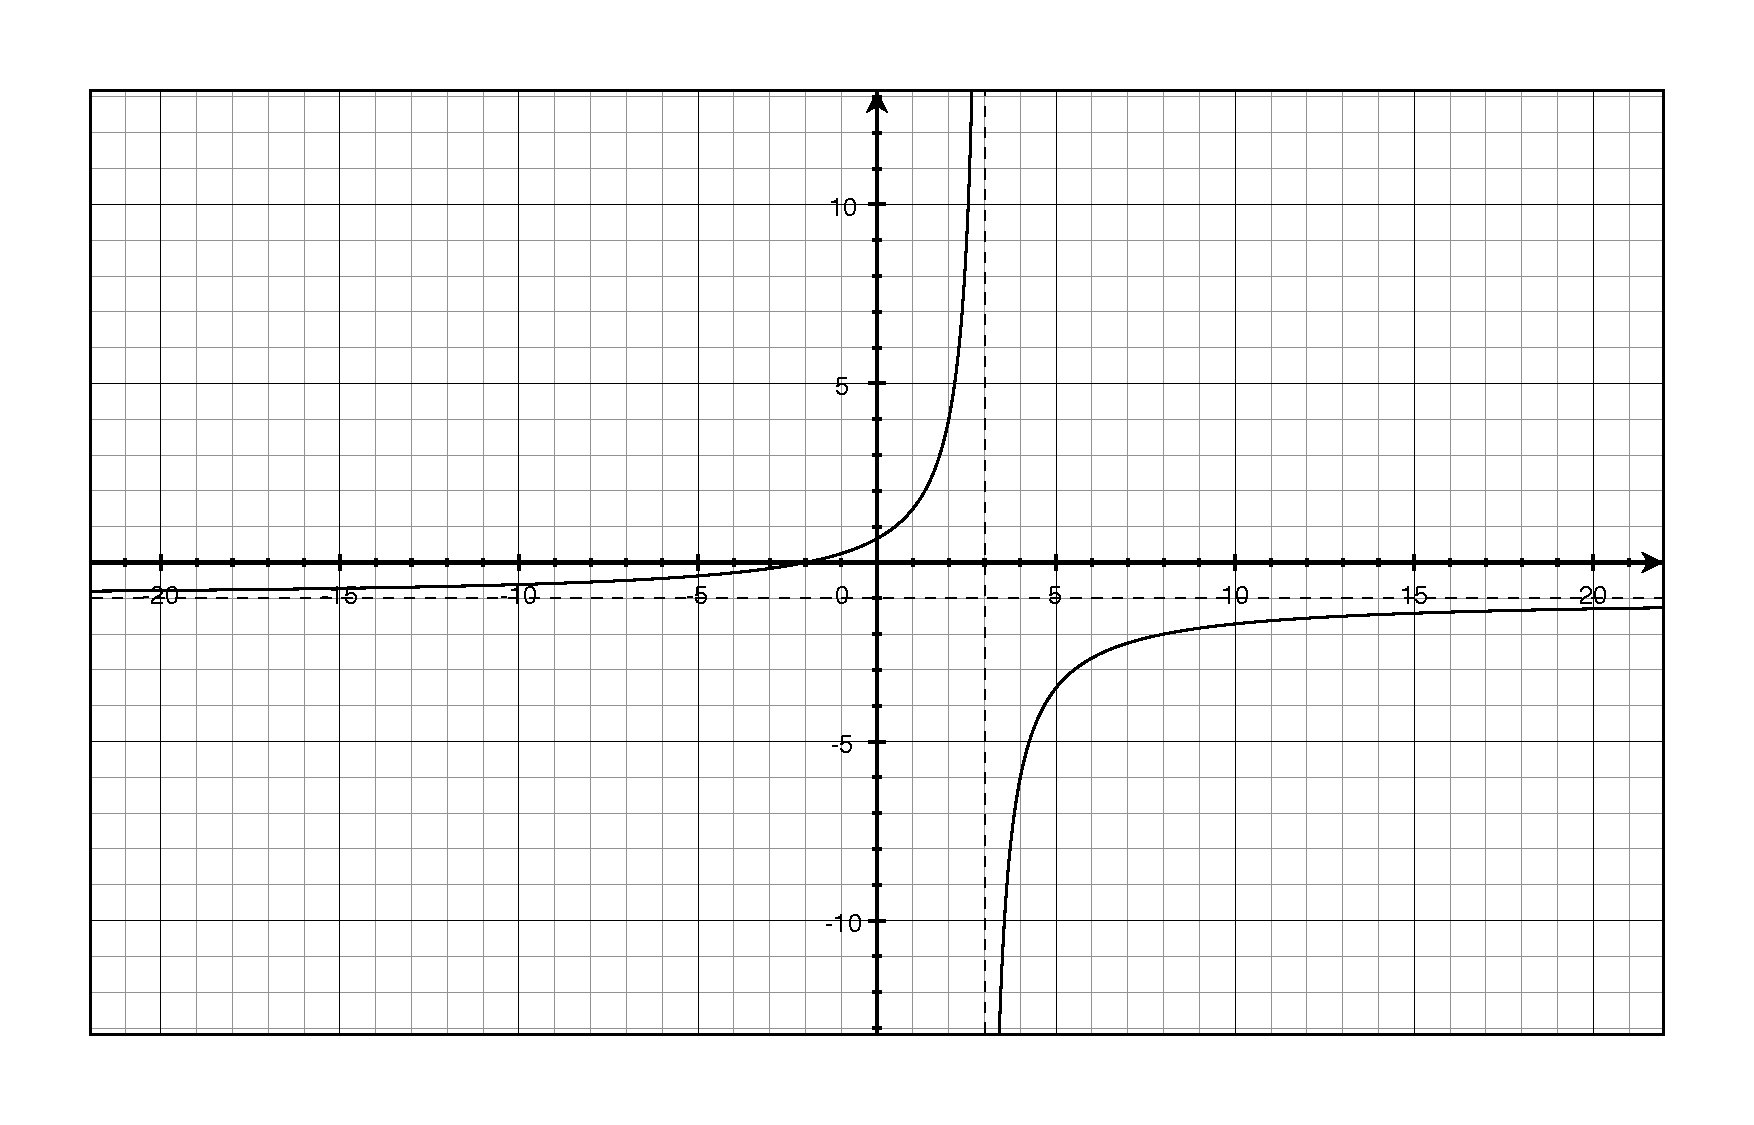
\includegraphics[scale=.6]{graph.eps}
\else
  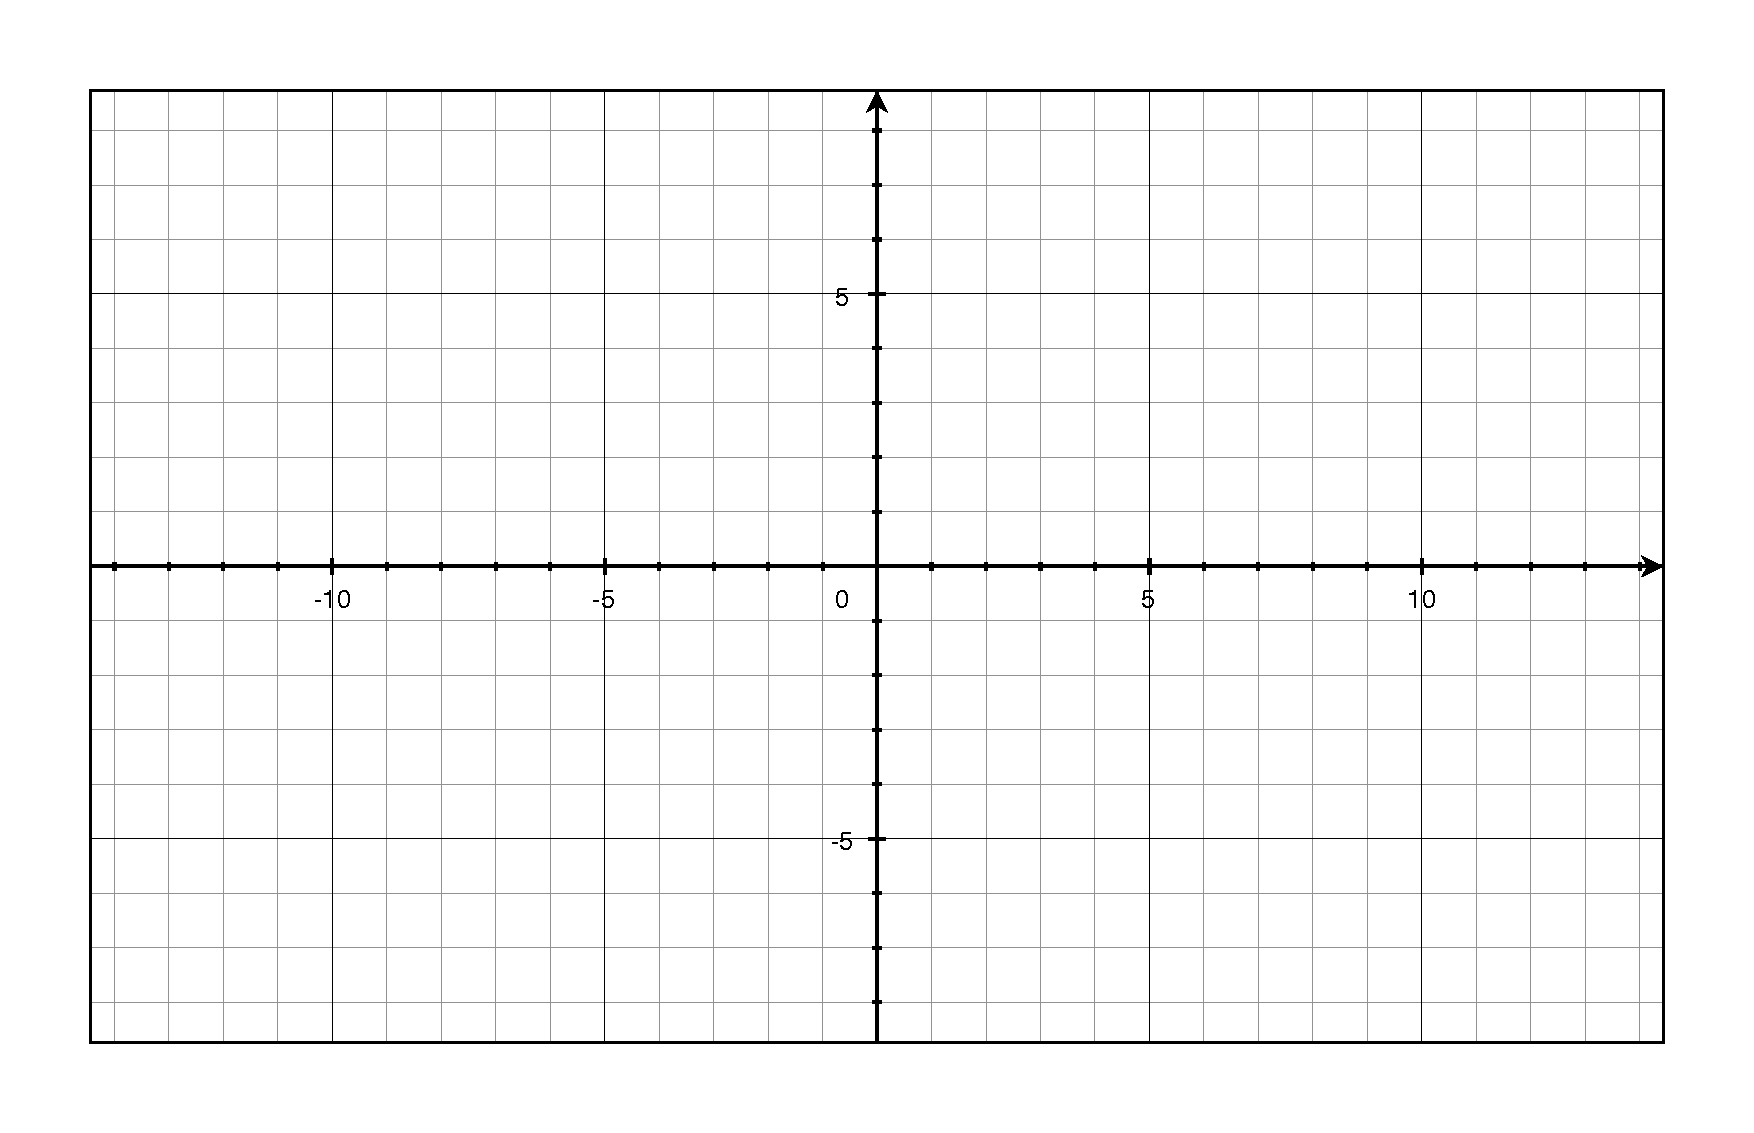
\includegraphics[scale=.6]{empty_grid.eps}
\fi
  \caption*{Question \ref{graph}}
\end{figure}


%% \question[15]
%% \[
%%   f(x) = \frac{-3x}{\sqrt{x^2 + 4}}
%% \]

%% \begin{solution}[9 cm]
%% \end{solution}

%% \begin{figure}[H]
%%   \centering
%%   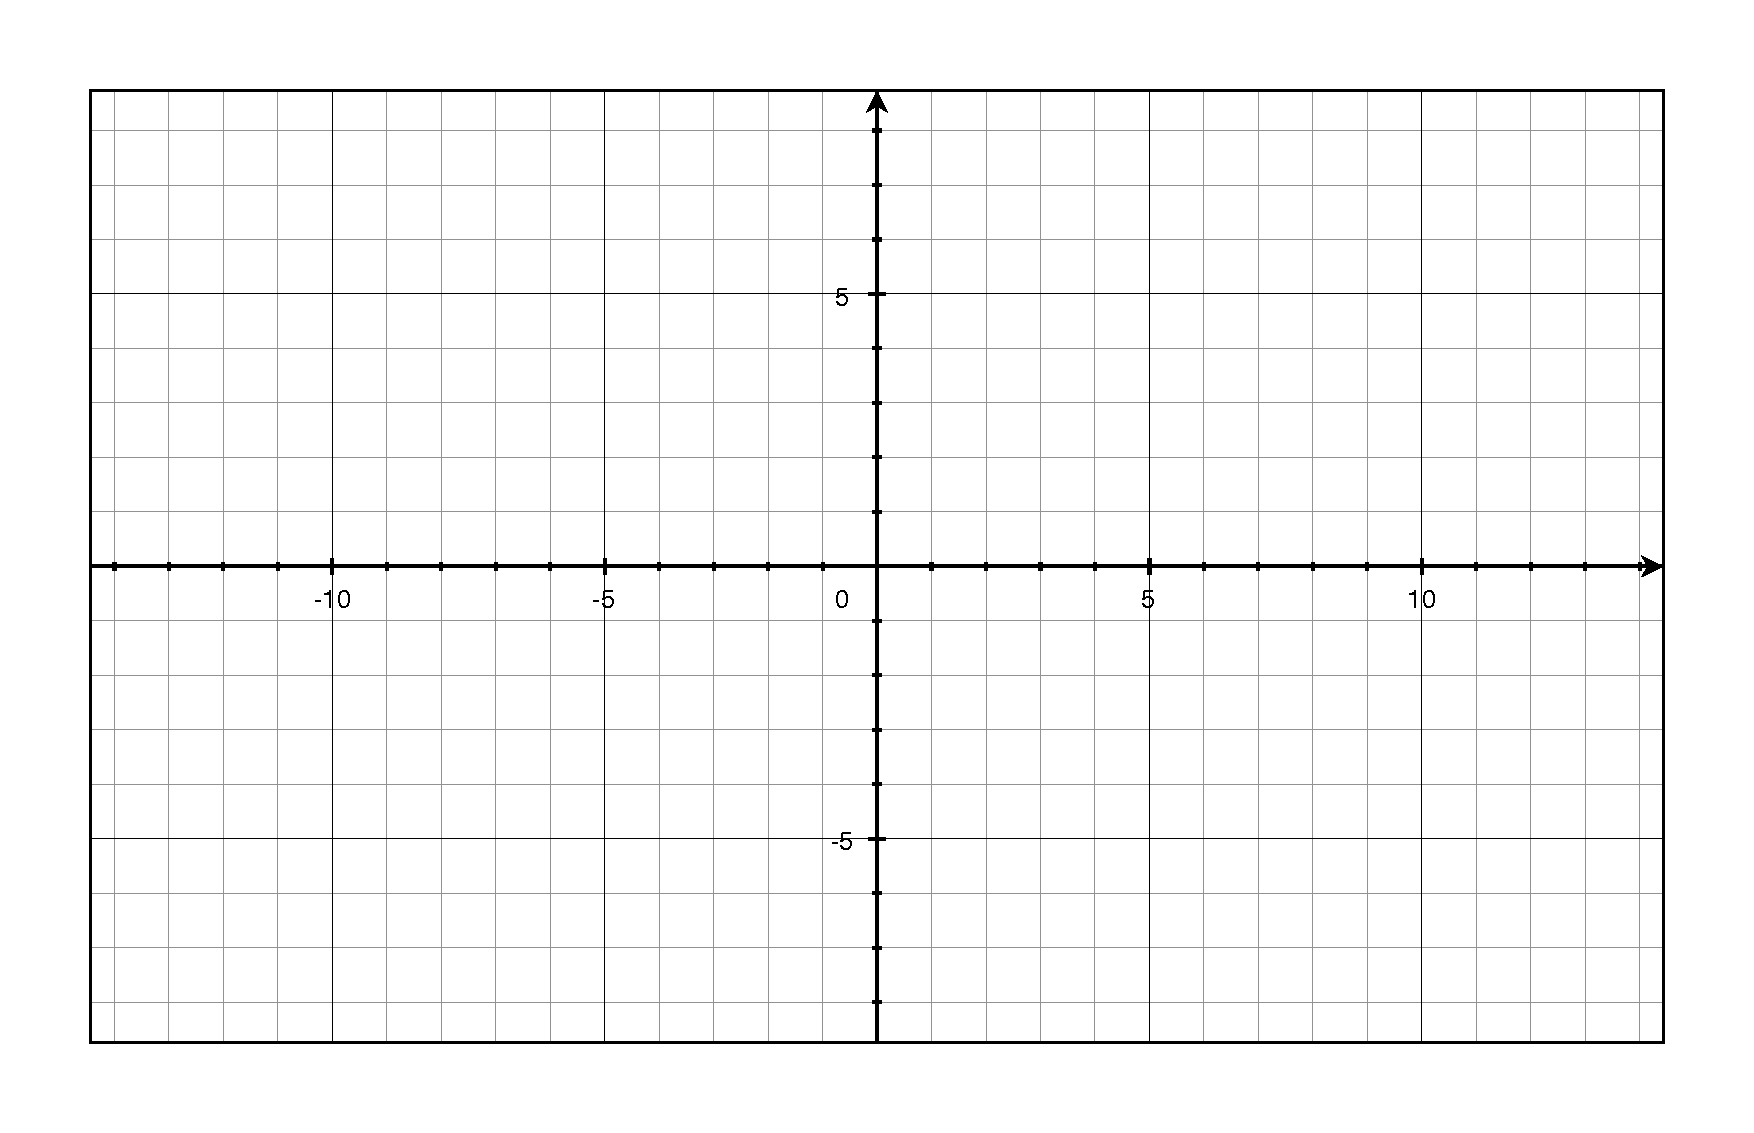
\includegraphics[scale=.5]{empty_grid.eps}
%%   \caption*{Question \ref{graph:last}}
%% \end{figure}

%% \question[10]
%% \label{graph:last}

%% Sketch the graph of a differentiable function that satisfies these conditions:
%% \begin{itemize*}
%% \item $f(0) = 1$; $f(2) = 3$; $f'(0) = f'(2) = 0$
%% \item $f'(x) > 0$ in $(0, 2)$ and $f'(x) < 0$  in $(-\infty, 0) \cup (2, 0)$
%% \item $f''(x) > 0$ in $(-\infty, 1)$ and $f''(x) < 0$  in $(1, \infty)$

%% \end{itemize*}

%% \begin{solution}[1 cm]
%% \end{solution}

%% \begin{figure}[H]
%%   \centering
%%   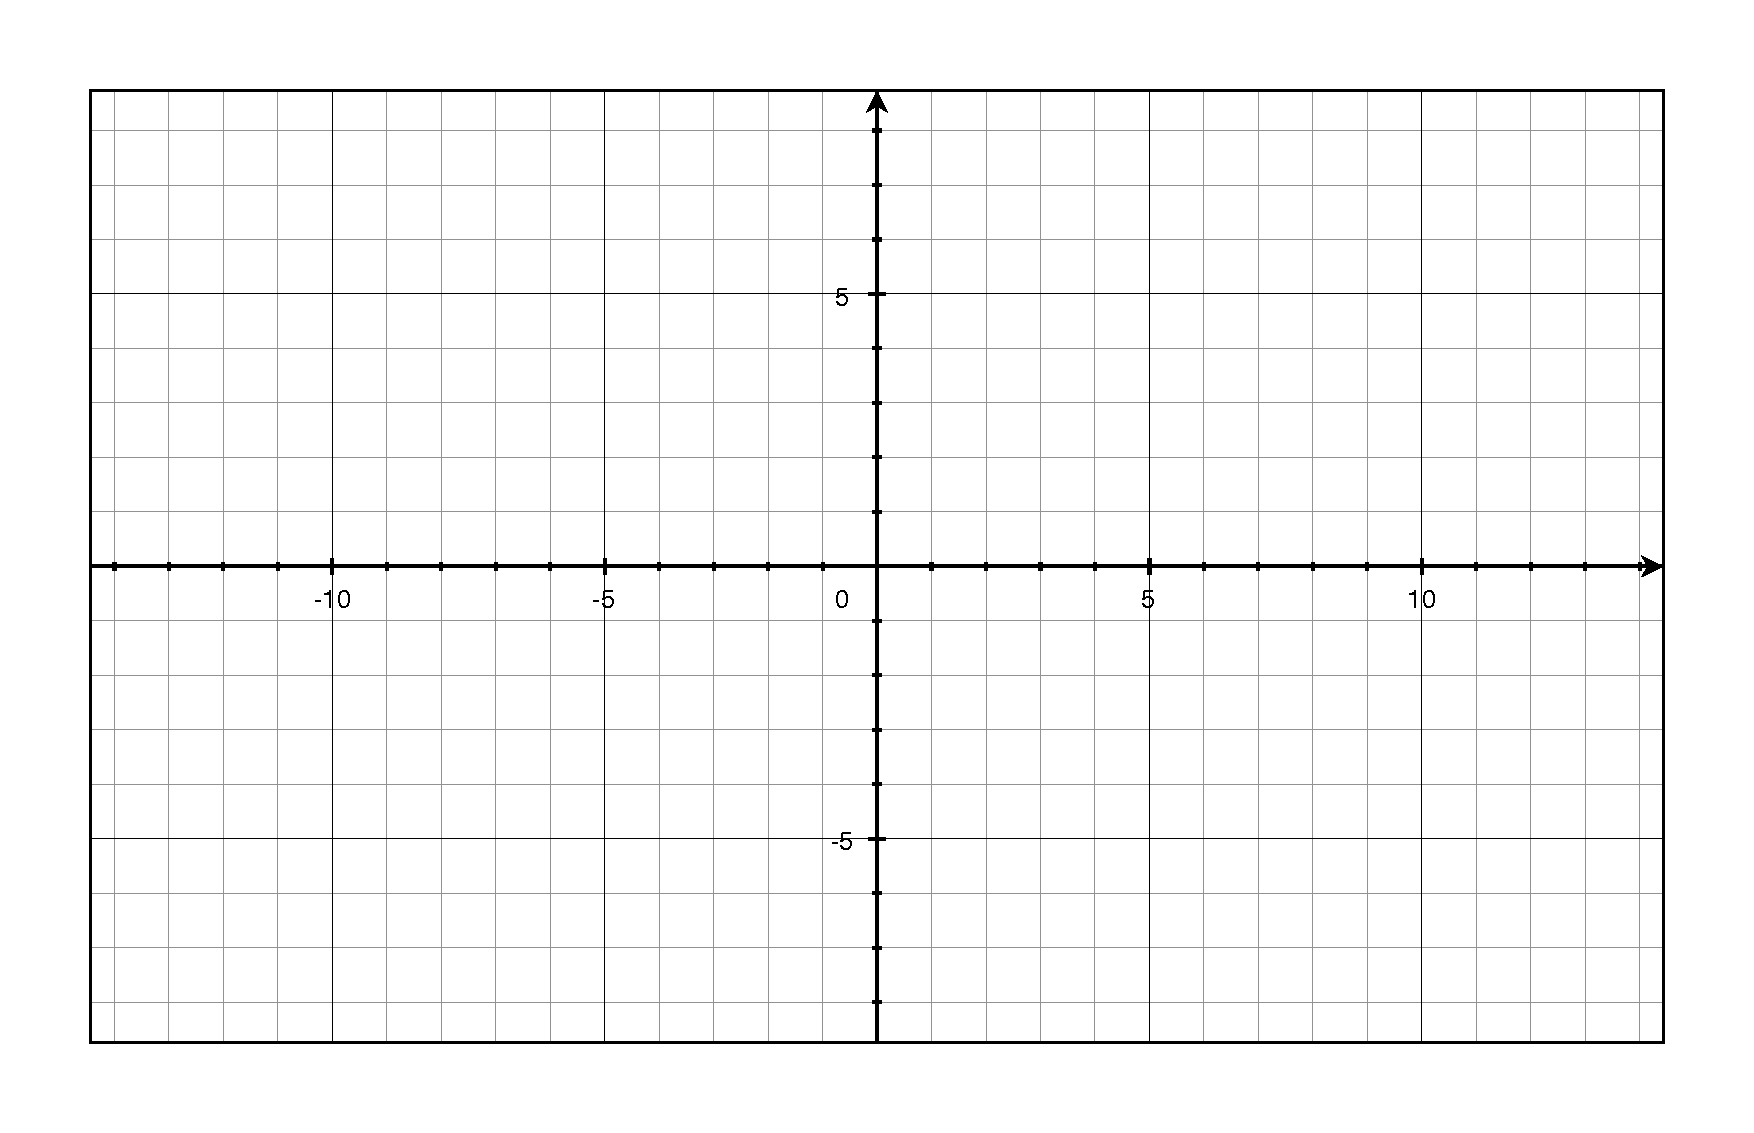
\includegraphics[scale=.5]{empty_grid.eps}
%%   \caption*{Question \ref{graph:last}}
%% \end{figure}

\pagebreak

\uplevel{\section{Extra Credit}}

\bonusquestion[10] A long rectangular sheet of metal, 12 inches wide, is to be made into a rain gutter by turning up two
sides at angles of $\theta$.

If $x$ is the number of inches to turn up which gives the gutter its greatest capacity, find an expression for $x$ in terms of $\theta$.

\begin{solution}
Since the length is fixed, the only way to maximize the volume is to maximize the area of the cross section.  If you
draw a picture, and let $x$ be the length of metal folded up on each side, you can see that this area is:
\begin{align*}
  A(x) &= (12 - 2x) \cdot x \sin \theta + x \sin \theta \cdot x \cos \theta \\
    &= 12 x \sin \theta - 2x^2 \sin \theta + x^2 \sin \theta \cos \theta \\
  A'(x) &= 12 \sin \theta - 2x^2 \sin \theta + x^2 \sin \theta \cos \theta \\
\\
  12 \sin \theta - 2x^2 \sin \theta + x^2 \sin \theta \cos \theta &= 0 \\
  x &= \frac{6}{1 - \cos \theta} \\
\\
\end{align*}

We can use the second derivative test to determine whether this is  aminimum or maximum:
\begin{align*}
  A''(x) &= -4 \sin \theta + 2 \sin \theta \cos \theta \\
-4 \sin \theta + 2 \sin \theta \cos \theta &< 0 \\
  \cos \theta &> -2 \\
\end{align*}

Since $A''$ is always negative any critical points are maxiumums.

\end{solution}

\end{questions}

\end{document}
